\section{Sprint 1 : Authentification et gestion des accès}

\subsection{Introduction}

Ce chapitre présente le premier Sprint de réalisation de la plateforme GMAO. Il est consacré à l'authentification des utilisateurs, à la gestion des comptes, des profils, des rôles et des autorisations.

Cette étape conditionne l'ensemble des fonctionnalités développées dans les Sprints suivants. En effet, l'accès aux machines, aux plans de maintenance, aux ordres de travail, aux stocks et aux documents techniques doit être réservé aux utilisateurs autorisés et adapté à leurs responsabilités.

Le chapitre expose les objectifs et le Sprint Backlog, puis présente la conception des mécanismes d'authentification et de contrôle d'accès. Il décrit ensuite les fonctionnalités réalisées, les dispositions de sécurité mises en place ainsi que les tests permettant de valider l'incrément produit.

\subsection{Objectifs du Sprint}

L'objectif principal de ce Sprint est de mettre en place un accès sécurisé à la plateforme et de permettre à l'administrateur de gérer les comptes utilisateurs.

Les objectifs spécifiques sont les suivants :

\begin{itemize}
    \item permettre l'inscription et la connexion locale des utilisateurs ;
    \item vérifier l'adresse électronique lors de la création d'un compte ;
    \item prendre en charge l'authentification à l'aide d'un compte Google ;
    \item gérer la réinitialisation des mots de passe ;
    \item maintenir les sessions au moyen de jetons d'accès et de rafraîchissement ;
    \item gérer les profils et les photographies des utilisateurs ;
    \item permettre à l'administrateur d'approuver, de rejeter ou de désactiver les comptes ;
    \item appliquer un contrôle d'accès fondé sur les rôles ;
    \item protéger les routes du frontend et les points d'entrée de l'API.
\end{itemize}

À la fin du Sprint, un utilisateur authentifié et approuvé doit pouvoir accéder uniquement aux fonctionnalités correspondant à son rôle.

\subsection{Sprint Backlog}

Le Sprint Backlog regroupe les éléments du Product Backlog sélectionnés pour ce Sprint ainsi que les tâches nécessaires à leur réalisation. Le tableau~\ref{tab:sprint1-backlog} recense ces tâches.

{\small
\setlength{\tabcolsep}{5pt}
\begin{longtable}{|p{1cm}|p{10.3cm}|p{1.5cm}|p{1.4cm}|}
\caption{Sprint Backlog du Sprint 1}
\label{tab:sprint1-backlog}\\
\hline
\textbf{ID} & \textbf{Tâche} & \textbf{Priorité} & \textbf{Statut} \\
\hline
\endfirsthead

\hline
\textbf{ID} & \textbf{Tâche} & \textbf{Priorité} & \textbf{Statut} \\
\hline
\endhead

S1-01 &
Mettre en place l'inscription et la vérification de l'adresse électronique. &
Haute & Réalisé \\
\hline

S1-02 &
Développer l'authentification locale et la gestion des sessions. &
Haute & Réalisé \\
\hline

S1-03 &
Mettre en place la récupération et la réinitialisation du mot de passe. &
Haute & Réalisé \\
\hline

S1-04 &
Intégrer l'authentification Google et la complétion du profil. &
Moyenne & Réalisé \\
\hline

S1-05 &
Développer la gestion des profils et des photographies. &
Moyenne & Réalisé \\
\hline

S1-06 &
Développer l'administration des utilisateurs et l'approbation des comptes. &
Haute & Réalisé \\
\hline

S1-07 &
Appliquer le contrôle d'accès fondé sur les rôles à l'API et au frontend. &
Haute & Réalisé \\
\hline

S1-08 &
Vérifier les mécanismes d'authentification et de sécurité par des tests. &
Haute & Réalisé \\
\hline
\end{longtable}}

\subsection{User Stories du Sprint}

Les fonctionnalités de ce Sprint sont décrites sous la forme des User Stories suivantes :

{\small
\begin{itemize}
    \item \textbf{US01 :} en tant que visiteur, je souhaite créer un compte et vérifier mon adresse électronique afin de pouvoir accéder à la plateforme ;
    \item \textbf{US02 :} en tant qu'utilisateur, je souhaite m'authentifier afin d'accéder aux fonctionnalités correspondant à mon rôle ;
    \item \textbf{US03 :} en tant qu'utilisateur, je souhaite récupérer mon mot de passe afin de retrouver l'accès à mon compte ;
    \item \textbf{US04 :} en tant qu'utilisateur, je souhaite gérer mon profil afin de maintenir mes informations à jour ;
    \item \textbf{US05 :} en tant qu'administrateur, je souhaite approuver ou rejeter les comptes afin de contrôler les accès à la plateforme ;
    \item \textbf{US06 :} en tant qu'administrateur, je souhaite attribuer des rôles afin de limiter les fonctionnalités accessibles à chaque utilisateur.
\end{itemize}}

\subsection{Conception du Sprint}

\subsubsection{Diagramme des cas d'utilisation}

Le diagramme de la figure~\ref{fig:usecase-auth} présente les principaux cas d'utilisation associés à l'authentification et à la gestion des accès. Il distingue trois acteurs : le visiteur, qui accède uniquement aux opérations d'inscription, de connexion et de récupération du mot de passe ; l'utilisateur authentifié, qui gère son profil et sa session ; et l'administrateur, qui hérite des capacités de l'utilisateur et dispose en plus de la gestion des comptes et des rôles.

\begin{figure}[H]
    \centering
    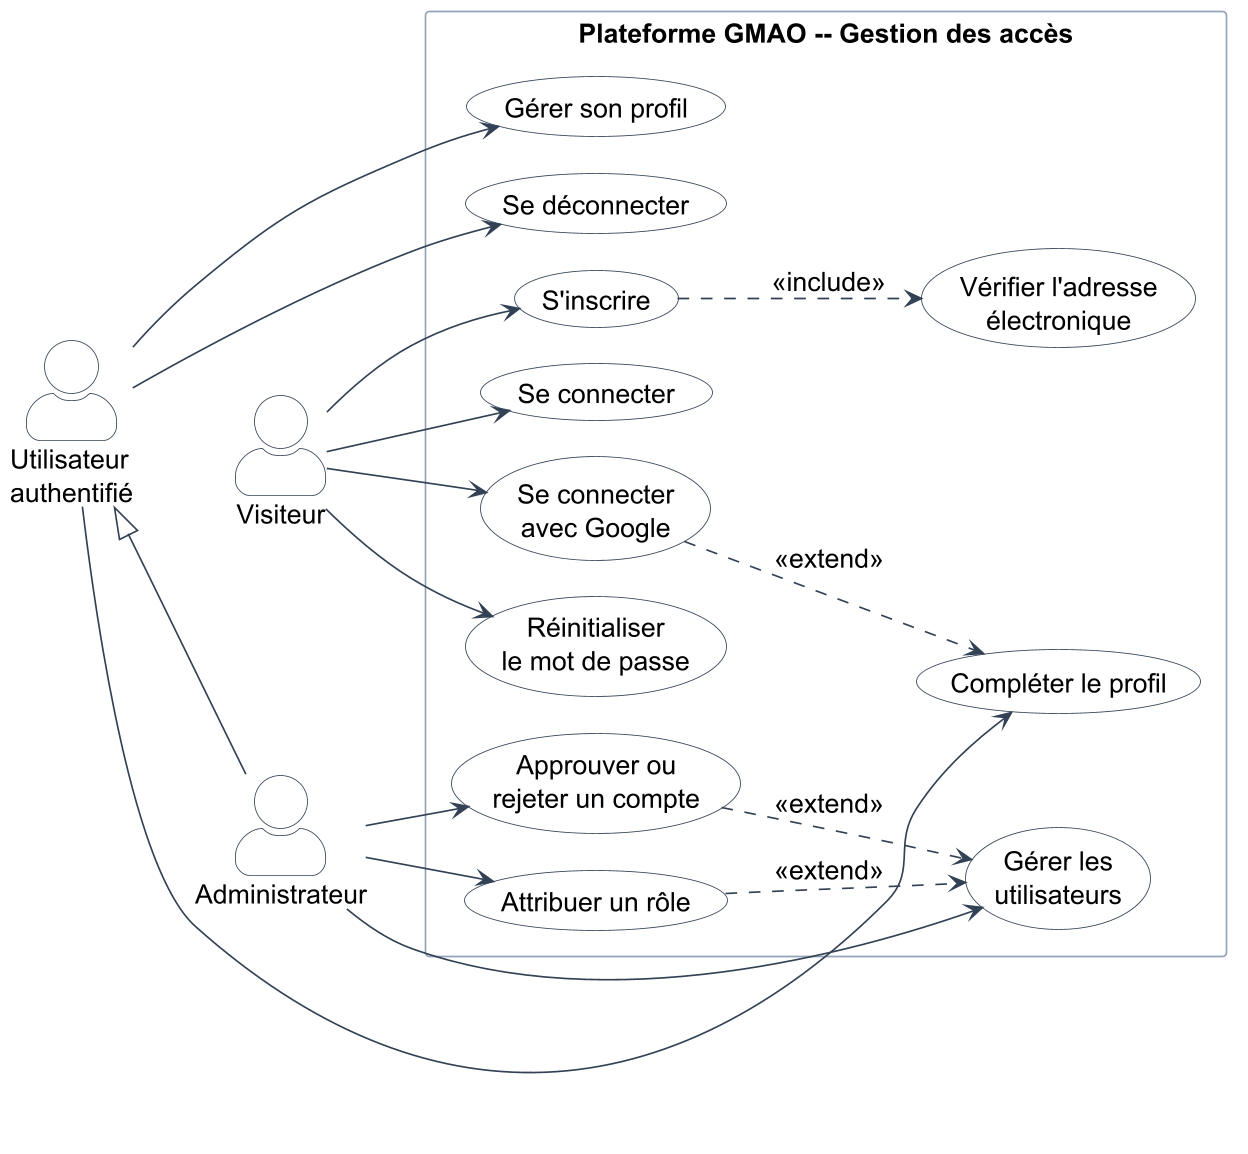
\includegraphics[width=0.78\textwidth,keepaspectratio]{figures/usecase-auth.png}
    \caption{Diagramme des cas d'utilisation du Sprint 1}
    \label{fig:usecase-auth}
\end{figure}

Les relations d'inclusion et d'extension traduisent les dépendances entre cas d'utilisation : l'inscription inclut la vérification de l'adresse électronique, tandis que la complétion du profil étend la connexion avec Google. L'approbation d'un compte et l'attribution d'un rôle étendent la gestion des utilisateurs.

\subsubsection{Diagramme de séquence de l'authentification}

La figure~\ref{fig:sequence-login} décrit le déroulement d'une authentification locale. Les identifiants sont transmis à l'API, qui vérifie le mot de passe, l'état du compte et le rôle avant de délivrer les jetons de session.

\begin{figure}[H]
    \centering
    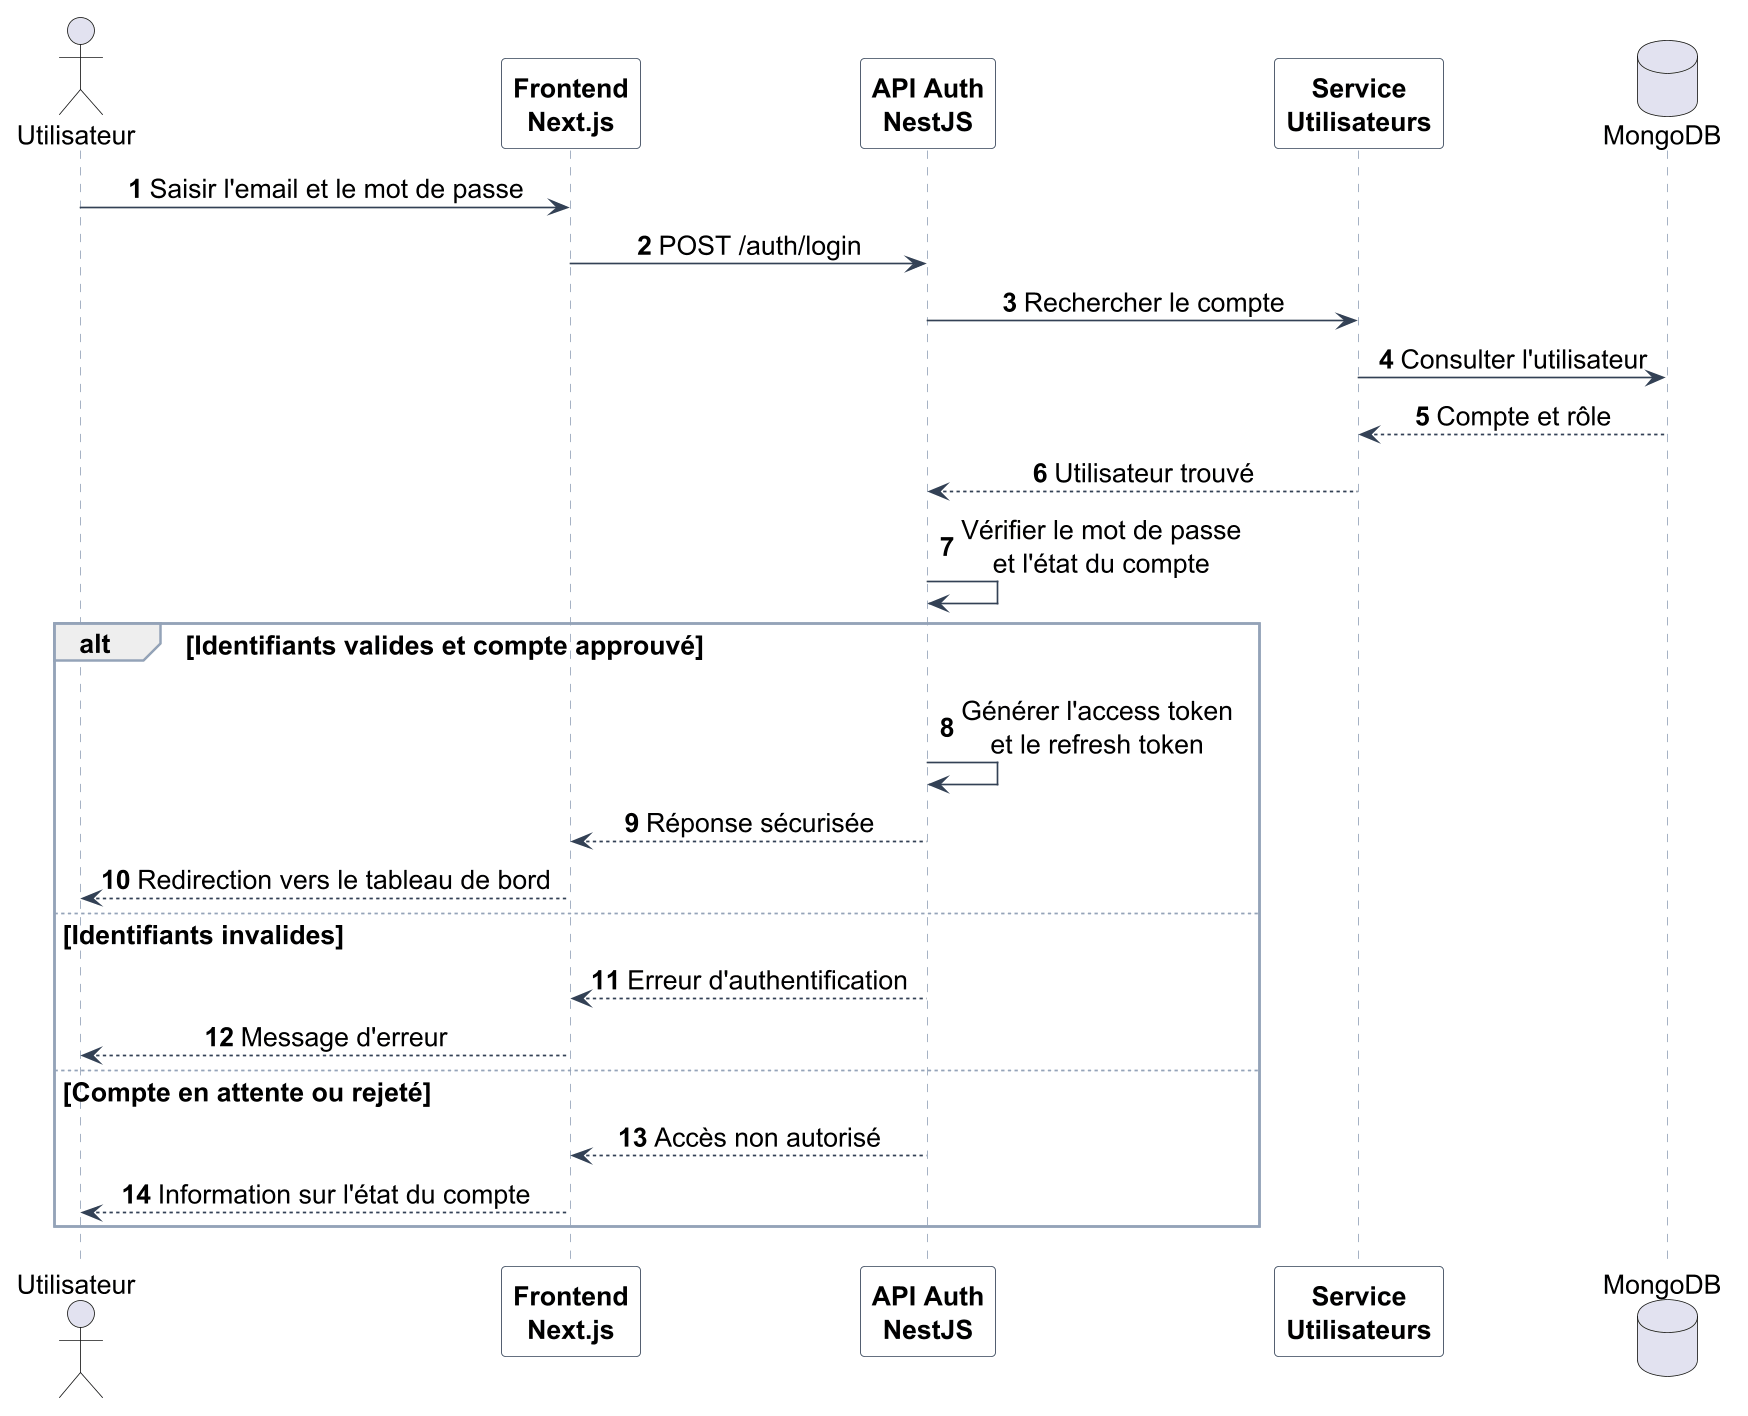
\includegraphics[width=\textwidth,height=0.72\textheight,keepaspectratio]{figures/sequence-login.png}
    \caption{Diagramme de séquence de l'authentification locale}
    \label{fig:sequence-login}
\end{figure}

Le scénario nominal conduit à la génération d'un jeton d'accès et d'un jeton de rafraîchissement, puis à la redirection vers le tableau de bord. Deux scénarios alternatifs sont pris en charge : des identifiants invalides, qui produisent un message d'erreur générique, et un compte encore en attente ou rejeté, qui se traduit par un refus d'accès explicite sans révéler d'information sur le compte.

\subsubsection{Modèle de données des utilisateurs}

La classe \texttt{User} centralise les informations d'identification, le rôle et l'état du compte. Les principaux champs sont présentés dans le tableau~\ref{tab:modele-user}.

\begin{table}[H]
\centering
\caption{Principaux champs de l'entité utilisateur}
\label{tab:modele-user}
\small
\begin{tabularx}{\textwidth}{|p{3.4cm}|p{2.5cm}|X|}
\hline
\textbf{Champ} & \textbf{Type} & \textbf{Rôle} \\
\hline
\texttt{user\_id} & Identifiant & Référence unique de l'utilisateur \\
\hline
\texttt{email} & Chaîne & Identifiant de connexion, unique \\
\hline
\texttt{nom\_complet} & Chaîne & Nom affiché dans l'application \\
\hline
\texttt{passwordHash} & Chaîne & Mot de passe chiffré avec bcrypt \\
\hline
\texttt{role} & Énumération & \texttt{ADMIN}, \texttt{TECHNICIAN} ou \texttt{OPERATOR} \\
\hline
\texttt{approvalStatus} & Énumération & En attente, approuvé ou rejeté \\
\hline
\texttt{isVerified} & Booléen & Indique si l'adresse électronique est vérifiée \\
\hline
\texttt{isActive} & Booléen & Permet de désactiver un compte \\
\hline
\texttt{photo} & Référence & Photographie de profil, facultative \\
\hline
\end{tabularx}
\end{table}

Les comptes créés par inscription sont initialement en attente d'approbation. La connexion n'est autorisée qu'après vérification de l'adresse électronique et validation par un administrateur. Les mots de passe ne sont jamais stockés en clair : seule leur empreinte bcrypt est conservée.

\subsection{Réalisation}

\subsubsection{Authentification locale}

Le formulaire d'authentification permet à l'utilisateur de saisir son adresse électronique et son mot de passe. Après validation côté client, les données sont transmises à l'API NestJS par une requête sécurisée.

Le service d'authentification vérifie successivement l'existence du compte, la validité du mot de passe, la vérification de l'adresse électronique, l'état d'approbation et l'activation du compte. En cas de succès, un jeton d'accès et un jeton de rafraîchissement sont générés.

Le jeton d'accès autorise les requêtes vers les points d'entrée protégés. Le jeton de rafraîchissement permet de maintenir la session et d'éviter une nouvelle saisie des identifiants à chaque expiration du jeton d'accès. Des messages d'erreur génériques sont affichés en cas d'échec afin de ne pas révéler si l'adresse électronique existe dans le système.

Le formulaire d'authentification regroupe la saisie des identifiants, l'accès par compte Google et le lien de récupération du mot de passe.

\begin{figure}[H]
    \centering
    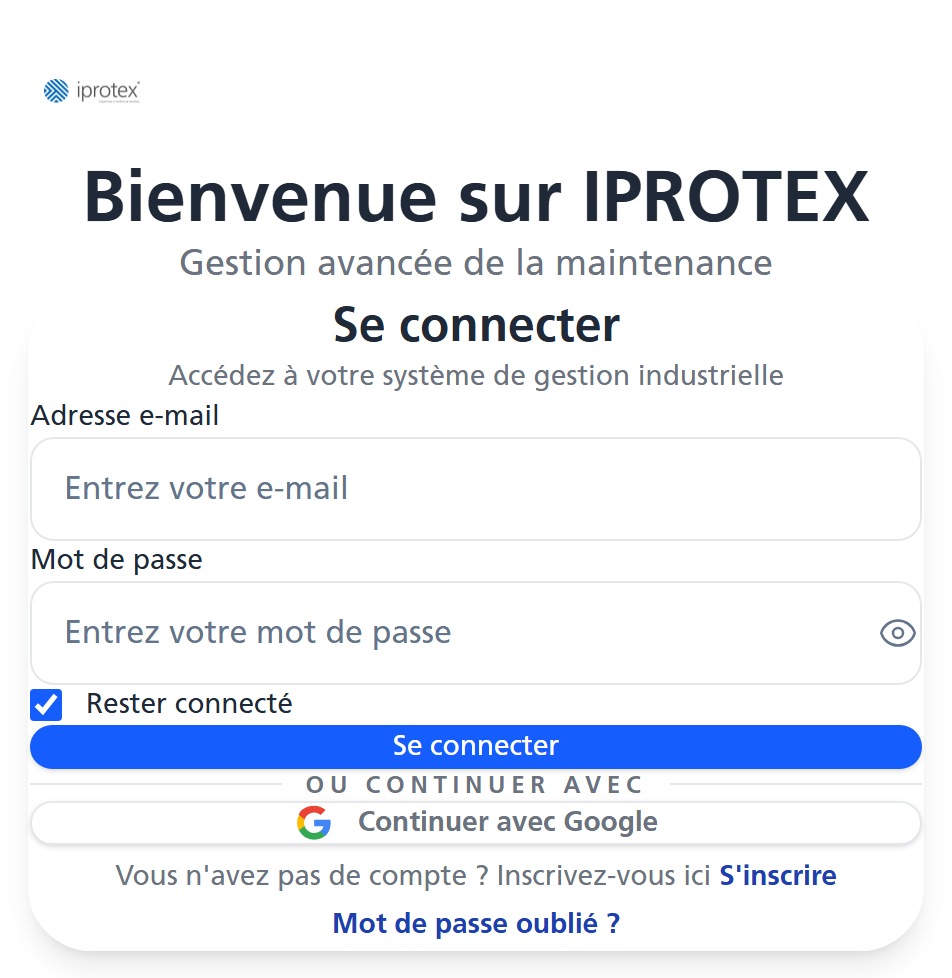
\includegraphics[width=0.52\textwidth,height=0.72\textheight,keepaspectratio]{figures/captures/sprint1-login.png}
    \caption{Interface d'authentification}
    \label{fig:sprint1-login}
\end{figure}
\subsubsection{Inscription et vérification de l'adresse électronique}

Le formulaire d'inscription permet de saisir le nom complet, l'adresse électronique, le mot de passe et la confirmation du mot de passe. Les données sont contrôlées avant leur enregistrement, notamment l'unicité de l'adresse électronique et la robustesse du mot de passe.

À la suite de l'inscription, un courriel contenant un lien de vérification est envoyé à l'utilisateur. La vérification de l'adresse électronique permet de confirmer que le demandeur contrôle bien la boîte de réception associée au compte.

Le compte est ensuite placé dans l'état d'attente d'approbation. Un administrateur examine la demande et peut l'approuver ou la rejeter. Cette double validation limite la création de comptes non autorisés et permet de contrôler l'accès aux données de maintenance.

\subsubsection{Authentification avec Google}

La plateforme prend également en charge l'authentification à l'aide d'un compte Google. Le mécanisme repose sur le protocole OAuth~2.0 et sur un échange sécurisé entre le fournisseur d'identité et le backend.

Lors de la première connexion, les informations nécessaires sont récupérées auprès du fournisseur d'identité. L'utilisateur complète ensuite son profil avant l'accès à la plateforme. Les comptes issus de Google restent soumis aux règles d'approbation et de contrôle des accès appliquées aux autres utilisateurs.

\subsubsection{Gestion du profil et des mots de passe}

L'utilisateur authentifié peut consulter et mettre à jour les informations de son profil, remplacer sa photographie et modifier les données autorisées.

Le mécanisme de récupération du mot de passe permet de saisir l'adresse électronique associée au compte. Un lien temporaire est ensuite transmis par courriel. Le jeton utilisé est limité dans le temps et invalidé après son utilisation. Un administrateur peut également imposer la réinitialisation du mot de passe d'un utilisateur.

\subsubsection{Administration des utilisateurs et approbation des comptes}

L'espace d'administration permet de consulter la liste des utilisateurs, de filtrer les comptes selon leur état, d'approuver ou de rejeter une demande et d'attribuer un rôle.

Les actions de validation peuvent être réalisées individuellement ou en masse. L'administrateur peut également désactiver un compte, réinitialiser un mot de passe et consulter les informations de profil.

Le tableau~\ref{tab:etats-compte} présente les principaux états d'un compte utilisateur.

\begin{table}[H]
\centering
\caption{États d'un compte utilisateur}
\label{tab:etats-compte}
\small
\begin{tabularx}{\textwidth}{|p{3cm}|X|}
\hline
\textbf{État} & \textbf{Signification} \\
\hline
Non vérifié & L'adresse électronique n'a pas encore été confirmée \\
\hline
En attente & L'adresse est vérifiée, mais le compte attend la décision de l'administrateur \\
\hline
Approuvé & Le compte peut accéder aux fonctionnalités correspondant à son rôle \\
\hline
Rejeté & La demande d'accès a été refusée \\
\hline
Désactivé & Un compte anciennement autorisé ne peut plus se connecter \\
\hline
\end{tabularx}
\end{table}

L'écran d'administration liste les comptes, permet de les filtrer par état et propose les actions d'approbation ou de rejet ainsi que l'attribution d'un rôle.

\begin{figure}[H]
    \centering
    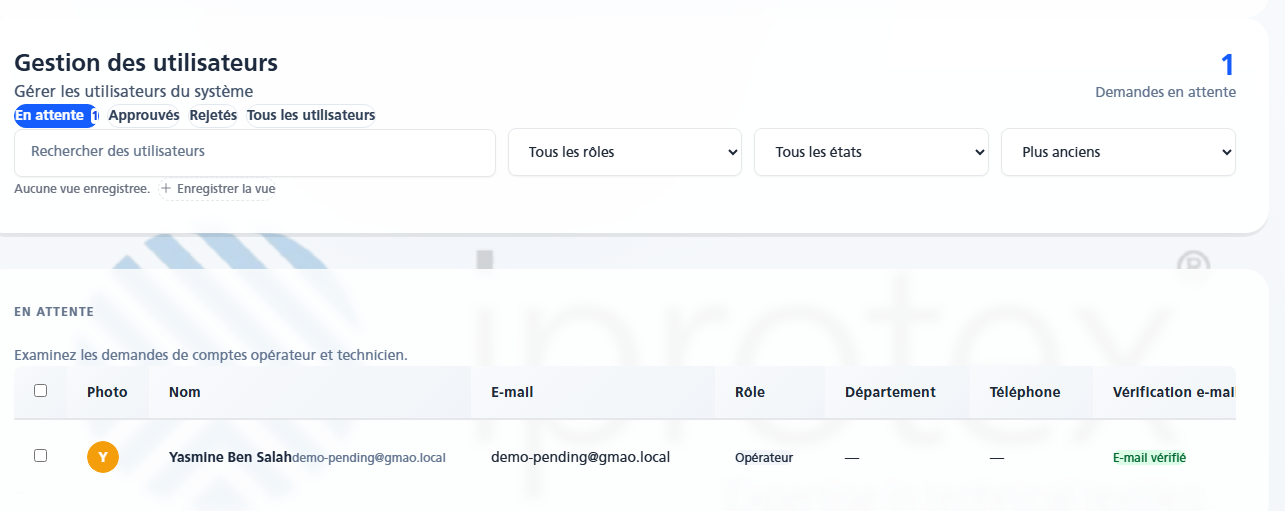
\includegraphics[width=0.90\textwidth,height=0.55\textheight,keepaspectratio]{figures/captures/sprint1-user-approval.png}
    \caption{Approbation des comptes utilisateurs}
    \label{fig:sprint1-user-approval}
\end{figure}
\subsubsection{Contrôle d'accès et sécurité}

Le contrôle d'accès repose sur trois rôles : \texttt{ADMIN}, \texttt{TECHNICIAN} et \texttt{OPERATOR}. Des gardes d'autorisation vérifient le jeton et le rôle avant toute opération protégée~\cite{nestjs_auth}. Le frontend applique également une protection des routes et adapte les menus aux habilitations de l'utilisateur.

Les dispositions de sécurité suivantes ont été mises en place :

\begin{itemize}
    \item chiffrement des mots de passe avec bcrypt~\cite{owasp_password} ;
    \item jetons JWT signés et durée de validité limitée~\cite{jwt_rfc7519} ;
    \item stockage du jeton de rafraîchissement dans un cookie sécurisé ;
    \item rotation, renouvellement et révocation des sessions ;
    \item validation des données reçues par l'API ;
    \item limitation du nombre de requêtes pour réduire les tentatives répétées ;
    \item configuration restrictive des origines autorisées ;
    \item en-têtes de sécurité HTTP et protection contre les injections de paramètres ;
    \item conservation des secrets dans les variables d'environnement du serveur ;
    \item vérification et approbation des comptes avant l'accès aux données.
\end{itemize}

\subsection{Tests et validation}

Les principales fonctionnalités du Sprint ont été vérifiées au moyen de tests fonctionnels, de tests d'API et de tests automatisés. Le tableau~\ref{tab:tests-sprint1} présente une synthèse des scénarios validés.

{\small
\setlength{\tabcolsep}{5pt}
\begin{longtable}{|p{0.9cm}|p{8.2cm}|p{5.4cm}|}
\caption{Scénarios de test du Sprint 1}
\label{tab:tests-sprint1}\\
\hline
\textbf{ID} & \textbf{Scénario} & \textbf{Résultat attendu} \\
\hline
\endfirsthead

\hline
\textbf{ID} & \textbf{Scénario} & \textbf{Résultat attendu} \\
\hline
\endhead

T1-01 &
Création d'un compte avec des données valides &
Compte créé et placé en attente de vérification \\
\hline

T1-02 &
Vérification de l'adresse électronique &
Adresse confirmée et compte placé en attente d'approbation \\
\hline

T1-03 &
Connexion avec des identifiants valides &
Jetons générés et accès autorisé selon le rôle \\
\hline

T1-04 &
Connexion avec un mot de passe incorrect &
Accès refusé sans révélation d'information sensible \\
\hline

T1-05 &
Connexion avant approbation &
Accès refusé avec indication de l'état du compte \\
\hline

T1-06 &
Accès à une page protégée sans jeton &
Redirection vers l'authentification \\
\hline

T1-07 &
Expiration du jeton d'accès &
Renouvellement de la session par le jeton de rafraîchissement \\
\hline

T1-08 &
Déconnexion &
Session invalidée et redirection vers la page de connexion \\
\hline

T1-09 &
Première connexion avec Google &
Récupération des informations et complétion du profil \\
\hline

T1-10 &
Accès d'un opérateur à une fonction d'administration &
Requête refusée par le contrôle des autorisations \\
\hline

T1-11 &
Réutilisation d'un lien de réinitialisation déjà utilisé &
Lien refusé \\
\hline

T1-12 &
Tentatives de connexion répétées &
Limitation des requêtes appliquée \\
\hline

\end{longtable}}

À l'issue de ces vérifications, les fonctionnalités prévues pour le Sprint ont été validées. Les anomalies détectées ont été corrigées avant la présentation de l'incrément.

\subsection{Revue du Sprint et conclusion}

Lors de la revue du Sprint, les mécanismes d'inscription, d'authentification, de récupération du mot de passe, de gestion du profil et d'administration des comptes ont été présentés. Le contrôle d'accès fondé sur les rôles a également été vérifié pour les trois profils de la plateforme.

Les principaux résultats obtenus sont les suivants :

\begin{itemize}
    \item mise en place d'un accès sécurisé et contrôlé à la plateforme ;
    \item intégration de l'authentification locale et de l'authentification Google~\cite{google_oauth} ;
    \item gestion des profils, des rôles et des états des comptes ;
    \item approbation des utilisateurs par l'administrateur ;
    \item protection des routes et des points d'entrée de l'API ;
    \item séparation des sessions d'accès et de rafraîchissement ;
    \item application effective des autorisations selon les rôles.
\end{itemize}

La rétrospective a confirmé l'intérêt de traiter ce module en premier, puisque les fonctionnalités développées dans les Sprints suivants reposent toutes sur l'identité et les autorisations des utilisateurs.

Le Sprint 2 sera consacré à la gestion des machines, des modules et des documents techniques.
